%% Linking VRscores to Compustat, step by step: instructions for polisy_triangulate.py
%% Compile with pdflatex, twice:  pdflatex Linkage_instructions.tex
%% Uses only standard packages (TeX Live, MiKTeX or Overleaf).
\documentclass[11pt,a4paper]{article}
\usepackage[T1]{fontenc}
\usepackage[utf8]{inputenc}
\usepackage{lmodern}
\usepackage{textcomp}
\usepackage{amsmath}
\usepackage[margin=2.3cm,headheight=14pt]{geometry}
\usepackage{microtype}
\usepackage{parskip}
\usepackage[dvipsnames,table]{xcolor}
\usepackage{array,booktabs,longtable}
\usepackage{ragged2e}
\usepackage{float}
\usepackage{caption}
\usepackage{fancyhdr}
\usepackage{listings}
\usepackage{tikz}
\usetikzlibrary{arrows.meta,positioning}
\usepackage[hyphens]{url}
\usepackage[colorlinks=true,linkcolor=RoyalBlue!70!black,urlcolor=RoyalBlue!70!black,
            pdftitle={Linking VRscores to Compustat, Step by Step},pdfauthor={Mit Desai},bookmarksnumbered=true]{hyperref}
\urlstyle{same}
\makeatletter\g@addto@macro\UrlBreaks{\do\_}\makeatother

\definecolor{navy}{RGB}{31,56,100}
\definecolor{rvtext}{RGB}{91,44,111}
\definecolor{codebg}{RGB}{246,247,250}
\newcommand{\RV}{\textcolor{rvtext}{\textit{Requires verification}}}
\newcommand{\file}[1]{\texttt{#1}}
\newsavebox{\keyboxsave}
\newenvironment{keybox}[1]{\par\smallskip\noindent\begingroup\setlength{\fboxsep}{8pt}\setlength{\fboxrule}{0.6pt}%
  \begin{lrbox}{\keyboxsave}\begin{minipage}{\dimexpr\linewidth-2\fboxsep-2\fboxrule\relax}\setlength{\parskip}{5pt}%
  \textbf{\large\textcolor{navy}{#1}}\par}
  {\end{minipage}\end{lrbox}\fcolorbox{navy!60}{navy!4}{\usebox{\keyboxsave}}\endgroup\par\smallskip}
\makeatletter
\newcommand{\condbreak}[1]{\par\penalty-100\begingroup\setlength{\dimen@}{#1}\dimen@ii\pagegoal
  \advance\dimen@ii-\pagetotal\ifdim\dimen@>\dimen@ii\ifdim\dimen@ii>\z@\vfil\fi\break\fi\endgroup}
\makeatother
\newcolumntype{L}[1]{>{\RaggedRight\arraybackslash\hspace{0pt}}p{#1}}
\lstset{basicstyle=\ttfamily\small,backgroundcolor=\color{codebg},frame=single,rulecolor=\color{navy!30},
        breaklines=true,columns=fullflexible,keepspaces=true,showstringspaces=false,upquote=true,
        xleftmargin=4pt,xrightmargin=4pt,aboveskip=6pt,belowskip=6pt}

\setcounter{secnumdepth}{1}
\renewcommand{\arraystretch}{1.25}
\captionsetup{font=small,labelfont=bf,skip=5pt}
\setlength{\LTpre}{4pt}\setlength{\LTpost}{6pt}
\tolerance=1000
\emergencystretch=3em
\raggedbottom

\pagestyle{fancy}
\fancyhf{}
\fancyhead[L]{\small\itshape Linking VRscores to Compustat, step by step}
\fancyhead[R]{\small\thepage}
\renewcommand{\headrulewidth}{0.4pt}
\fancypagestyle{plain}{\fancyhf{}\fancyfoot[C]{\small\thepage}\renewcommand{\headrulewidth}{0pt}}

\title{\vspace{-0.8cm}\textbf{Linking VRscores to Compustat, Step by Step}\\[6pt]
\large How to run the triangulated, audited linkage (\texttt{polisy\_triangulate.py})}
\author{Mit Desai\\[2pt]\small Prepared for the Research Team}
\date{14 October 2026}

\begin{document}
\maketitle
\thispagestyle{plain}

\begin{keybox}{What you will do, in one box}
\begin{enumerate}\setlength{\itemsep}{2pt}
\item Put \file{polisy\_triangulate.py} in your \textbf{POLISY} folder in Google Drive and open \file{POLISY\_linkage.ipynb} in Colab.
\item \textbf{Step A.} Build the links. The code checks every VRscores-to-Compustat link against independent sources and labels it by how it was confirmed. A few minutes.
\item \textbf{Review.} Decide by hand the few links whose sources disagree, in a spreadsheet. Rebuild.
\item \textbf{Steps B and C.} Two people check a random sample of 200 links, separately and blind. The code turns their answers into an error rate with a 95\% interval.
\item \textbf{Steps D and E.} Only now are political data read: the code compares linked and unlinked firms and writes one workforce panel per link set.
\item \textbf{Step F.} In Stata, run the thesis model once per link set. If the coefficient barely moves, the matching does not drive the result.
\end{enumerate}
Everything the code writes goes to \textbf{POLISY/linkage} in Google Drive. Nothing is lost when Colab disconnects.
\end{keybox}

\tableofcontents

%% ======================================================================
\section{What the code does}\label{sec:what}

\textbf{The problem.} DIPI is keyed by GVKEY, so it joins Compustat exactly. VRscores' public files identify employers only by an anonymous ID and a name. The one uncertain step in the DIPI + VRscores design is therefore \emph{VRscores employer $\to$ Compustat firm}. Until now that step was a name match (POLISY module~04), which reviewers may call ``fuzzy matching''.

\textbf{The idea}, borrowed from Akcigit and Goldschlag (2025): trust a link when \emph{independent} sources reach the same firm, label every link by how it was confirmed, show who gets linked, and measure the error rate by hand. Figure~\ref{fig:triangle} shows the three sources.

\begin{figure}[H]
\centering
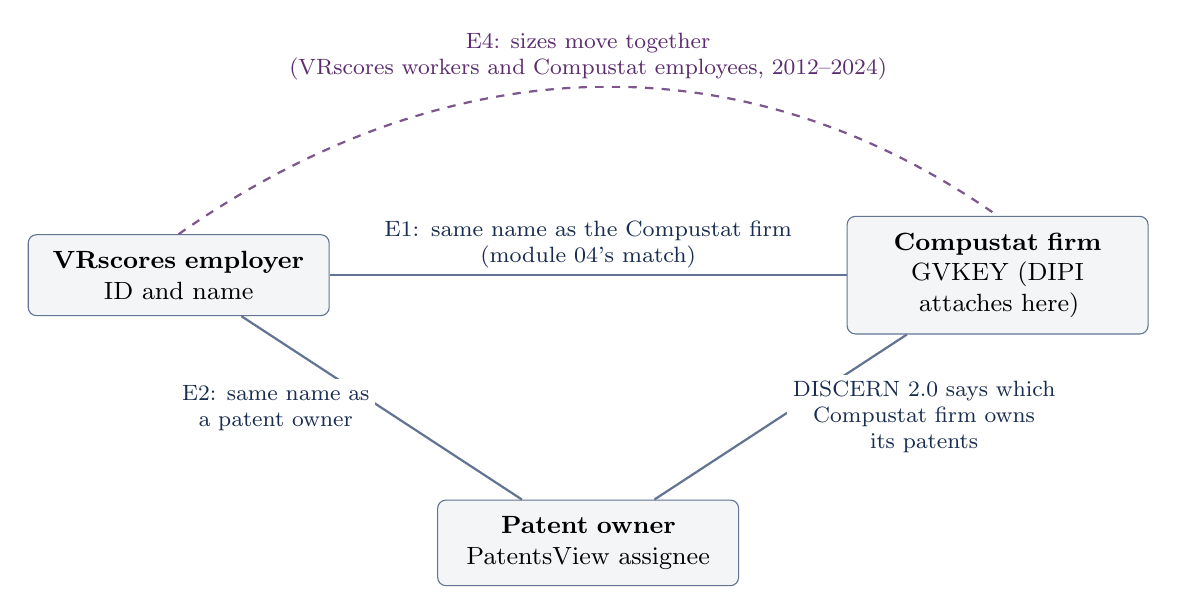
\begin{tikzpicture}[font=\small,
  node/.style={draw=navy!70,fill=navy!5,rounded corners=3pt,align=center,text width=3.4cm,inner sep=6pt},
  arr/.style={thick,draw=navy!70},
  lbl/.style={font=\footnotesize,text=navy!80!black,fill=white,inner sep=2pt,align=center}]
\node[node] (vr) at (0,0) {\textbf{VRscores employer}\\ID and name};
\node[node] (cs) at (10.4,0) {\textbf{Compustat firm}\\GVKEY (DIPI attaches here)};
\node[node] (pa) at (5.2,-3.4) {\textbf{Patent owner}\\PatentsView assignee};
\draw[arr] (vr) -- node[lbl,above,text width=5.2cm]{E1: same name as the Compustat firm\\(module 04's match)} (cs);
\draw[arr] (vr) -- node[lbl,left=2pt]{E2: same name as\\a patent owner} (pa);
\draw[arr] (pa) -- node[lbl,right=2pt]{DISCERN 2.0 says which\\Compustat firm owns\\its patents} (cs);
\draw[arr,dashed,draw=rvtext!80] (vr.north) to[out=35,in=145] node[lbl,above,text=rvtext]{E4: sizes move together\\(VRscores workers and Compustat employees, 2012--2024)} (cs.north);
\end{tikzpicture}
\caption{Three independent ways to reach the same firm. E3 (not drawn) is DISCERN's own list of each firm's names and subsidiaries.}\label{fig:triangle}
\end{figure}

\textbf{The evidence for each pair} (one VRscores employer, one GVKEY):
\begin{itemize}\setlength{\itemsep}{2pt}
\item \textbf{E1, Compustat name.} Module 04 matched the names (high or medium tier). The name must also be unique: no other Compustat firm has it, and the employer holds at least 90\% of the workers of all VRscores employers with the same cleaned name.
\item \textbf{E2, patent route.} The employer's name equals a patent owner's name, and DISCERN gives at least 80\% of that owner's patents (granted 2008--2021) to this GVKEY.
\item \textbf{E3, DISCERN names.} The name is on DISCERN's list of this firm's names and subsidiaries, and on no other firm's list.
\item \textbf{E4, size.} VRscores' matched workers fit Compustat's employees: a median ratio between 0.2\% and 150\% (module 04's rule), no jump of more than 3 times from one year to the next (a merger or split), and no movement in opposite directions.
\end{itemize}
E2 and E3 both come from DISCERN, so they count as one source. There are three independent sources: Compustat names, DISCERN, and sizes.

\textbf{Match types and link sets.} Table~\ref{tab:types} lists the labels. The analysis uses four nested sets: \emph{strict} (name and patent route agree), \emph{main} (two independent sources agree), \emph{broad} (main plus hand-accepted links and one-source links of module 04's high tier) and \emph{baseline} (module 04's rule as module 06 uses it today, for comparison). Every set links each employer to one firm only. An employer whose sources disagree stays out of every set until someone decides.

\begin{longtable}{@{}L{3.6cm}L{8.2cm}L{3.2cm}@{}}
\caption{Match types, in the order the code assigns them}\label{tab:types}\\
\toprule
\textbf{Match type} & \textbf{Meaning} & \textbf{In which sets}\\
\midrule\endfirsthead
\toprule
\textbf{Match type} & \textbf{Meaning} & \textbf{In which sets}\\
\midrule\endhead
\bottomrule\endfoot
rejected & rejected by hand & none\\
superseded & another firm was accepted by hand for this employer & none\\
conflict & the sources reach different firms: a person must decide & none (baseline only, as today)\\
triangulated\_patents & E1 and E2 reach the same firm & strict, main, broad\\
triangulated\_names & E1 and E3 & main, broad\\
name\_and\_size & E1 and E4 (no patents under the name in 2008--2021) & main, broad\\
discern\_and\_size & E2 or E3, and E4, without E1 (subsidiaries and renamed firms, e.g.\ Google LLC $\to$ Alphabet) & main, broad\\
hand\_accepted & accepted by hand, no two-source confirmation & broad\\
single\_source & one source only & broad if module 04's tier is high\\
\end{longtable}

\begin{keybox}{The one rule that matters most}
\textbf{No political variable is used to choose links.} Step~A reads only names, years, worker counts, Compustat sizes, patents and DISCERN. It refuses to read a VRscores column that looks political. Party data are read only in steps D and E. Those steps check a fingerprint (hash) of the frozen links file and stop if anyone has edited it. Hand decisions and audit coding use names, sizes, websites and 10-K subsidiary lists only. Do not run any regression with the new links before the audit (step C) is finished.
\end{keybox}

%% ======================================================================
\section{Before you start}\label{sec:before}

\textbf{The files I give you}, and where they go:
\begin{itemize}\setlength{\itemsep}{2pt}
\item \file{polisy\_triangulate.py}: the code. Upload it to your \textbf{POLISY} folder in Google Drive (the folder that holds \file{data}, \file{lab} and \file{polisy\_da}).
\item \file{POLISY\_linkage.ipynb}: the notebook. Upload it anywhere in Drive, double-click it, and choose \emph{Open with Google Colaboratory}.
\item \file{linkage\_sensitivity.do}: the Stata template for step F (the code also writes a copy to POLISY/linkage).
\end{itemize}

\textbf{The inputs the code reads.} You already made all of them with the lab notebook. The notebook's first cell lists each one as \emph{found} or \emph{MISSING}.

\begin{longtable}{@{}L{4.0cm}L{4.8cm}L{4.1cm}L{2.0cm}@{}}
\caption{Inputs, and what makes them}\label{tab:inputs}\\
\toprule
\textbf{Input} & \textbf{Where in Drive} & \textbf{Made by} & \textbf{Needed for}\\
\midrule\endfirsthead
\toprule
\textbf{Input} & \textbf{Where in Drive} & \textbf{Made by} & \textbf{Needed for}\\
\midrule\endhead
\bottomrule\endfoot
VRscores employer panel & \path{POLISY/polisy_da/data/canonical/vr_employer.parquet} & lab notebook cell 3 with \texttt{RUN\_POLISY\_DA = True} & A, E\\
Module 04's name match & \path{POLISY/polisy_da/data/keys/cw_vrid_gvkey.csv} & the same cell 3 & A\\
Compustat annual file & \path{POLISY/data} (your WRDS file) & you & A, D\\
Patents and their owners & \path{POLISY/lab/canonical/patents.parquet} and \path{POLISY/lab/staged/patentsview/g_assignee_disambiguated.parquet} & lab notebook cell 6b with \texttt{RUN\_PATENT\_LAYER = True} & A (E2)\\
DISCERN patent owners & \path{POLISY/lab/canonical/discern_patents.parquet} & cell 6b, from your DISCERN files & A (E2)\\
DISCERN name list & \path{POLISY/lab/staged/discern/names.parquet} & cell 6b (optional) & A (E3)\\
DIPI & \path{POLISY/polisy_da/data/canonical/dipi.parquet} & cell 3 (module 01 or 07) & D only\\
Firm-year patent panel & \path{POLISY/lab/panels/firm_patents_year.parquet} & cell 6b (optional) & D only\\
\end{longtable}

\textbf{If something is MISSING.} Open the lab notebook (\file{POLISY\_AI\_Innovation\_Lab}), run cells 1 and 2, then cell~3 with \texttt{RUN\_POLISY\_DA = True}. Then run cell~6b with \texttt{RUN\_PATENT\_LAYER = True}; its first run takes tens of minutes. Without the patent layer, step~A still runs, but only on names and sizes (no E2 or E3, and the strict set is empty).

%% ======================================================================
\section{Step 1: set up and check the inputs}\label{sec:setup}

Run the notebook's first cell. It installs two packages, connects Google Drive (approve the pop-up), loads the code from your POLISY folder and prints a table of the inputs. Every line needed for step~A should say \texttt{found}.

If your POLISY folder is not at \file{MyDrive/POLISY}, change the line \texttt{BASE = ...}. If the Compustat file is MISSING (for example because it sits in another folder), remove the \texttt{\#} in front of this line, write your file's path and run the cell again:
\begin{lstlisting}[language=Python]
tri.PATHS["compustat"] = BASE / "data" / "Compustat_Final.csv"
\end{lstlisting}

%% ======================================================================
\section{Step A: build the links}\label{sec:build}

Run the second code cell. Expect a few minutes, most of it spent reading the large files from Google Drive. In a test at the size of the real files (6.2 million employer-years, 4 million patents), the work itself took 19 seconds and stayed under 3.1 GB of memory, and Colab has about 12 GB. Read these printed lines:

\begin{longtable}{@{}L{4.4cm}L{10.6cm}@{}}
\toprule
\textbf{Line starts with} & \textbf{What it tells you}\\
\midrule\endhead
\bottomrule\endfoot
\texttt{VRscores:} & how many employers share a cleaned name with another (these cannot be linked by name alone)\\
\texttt{route 1} & module 04's pairs by tier, and how many you already decided by hand\\
\texttt{patent route:} & how many patent owners share a name with a VRscores employer and have one dominant DISCERN owner\\
\texttt{review list:} & how many pairs need a person (next section)\\
\texttt{match types:} & the count of each label in Table~\ref{tab:types}\\
\texttt{set strict / main / ...} & how many employer-firm links and firms each set holds\\
\texttt{links frozen as version} & the version number and fingerprint (hash) of this build; every rebuild with different results gets a new version, recorded in \file{linkage\_log.csv}\\
\end{longtable}

The cell then shows three tables, also saved in POLISY/linkage:
\begin{itemize}\setlength{\itemsep}{2pt}
\item \file{T1\_match\_types.csv}: pairs, employers, firms and matched workers by match type.
\item \file{T1b\_link\_sets.csv}: the same for each link set, with its share of all VRscores matched workers and how many employers each firm has.
\item \file{T3\_agreement.csv}: how often independent sources agree.
\end{itemize}

\textbf{Two checks before you go on.}
\begin{enumerate}\setlength{\itemsep}{2pt}
\item In \file{T3\_agreement.csv}, the first row (name-matched links whose name also has a dominant patent owner: does the patent route reach the same firm?) should be high. Disagreements there are mostly parents versus listed subsidiaries. A very low share means something upstream is wrong, for example DISCERN's firm codes not mapped to GVKEY. Stop and look before continuing. What counts as ``high'' is not known in advance (\RV); I would expect well above 80\%.
\item The strict set should contain most of the large patenting firms you know are in DIPI. Pick ten and search for them in \file{links\_all.csv} (open it in Google Sheets; do not save it).
\end{enumerate}

\textbf{Never edit \file{links\_all.csv}.} Its fingerprint is recorded in \file{protocol.json}, and steps D and E refuse to run if it changes. Decisions go in a separate file (next section).

%% ======================================================================
\section{Hand review: decide the pairs the sources could not settle}\label{sec:review}

\file{review\_list.xlsx} lists two kinds of pairs: \emph{conflicts}, where one employer reaches two firms (both rows are listed), and \emph{single-source} pairs that would enter the broad or baseline set. The largest employers come first, so the pairs that matter most are on top.

\begin{enumerate}\setlength{\itemsep}{3pt}
\item In Google Drive, open \textbf{POLISY/linkage/review\_list.xlsx}. Download it to use Excel, or open it with Google Sheets. The sheet \emph{How to decide} repeats these rules.
\item In the sheet \emph{Review}, fill the yellow columns for each row:
  \begin{itemize}\setlength{\itemsep}{1pt}
  \item \textbf{accept}: 1 if it is the same company, or a division or subsidiary the Compustat firm owned during 2012--2021; 0 if not. Leave it empty when unsure.
  \item \textbf{decided\_by}: your initials.
  \item \textbf{note}: where you checked, for example ``10-K 2016 Exhibit 21''.
  \end{itemize}
  For a conflict, accept the right firm (1) and reject the other (0). When the choice is between a parent and its listed subsidiary, accept the firm the thesis studies: the one with DIPI scores.
\item Decide on names, sizes, company websites and 10-K subsidiary lists only (SEC EDGAR full-text search finds Exhibit~21). \textbf{Never look at party, donation, DIPI or VRscores share data while deciding.}
\item Save the file in \textbf{POLISY/linkage} as \textbf{hand\_decisions.xlsx}. In Google Sheets: \emph{File $\to$ Download $\to$ Microsoft Excel}, then upload it to POLISY/linkage under that name. A later round goes in \file{hand\_decisions\_2.xlsx}, and so on. The code reads them all, and a later file overrides an earlier one.
\item Run step~A again with a note: \texttt{tri.build\_links(note="after review round 1")}. The review list now holds only the pairs still undecided. One round is usually enough. Pairs left undecided simply stay out of the main set.
\end{enumerate}

Your existing name-match review (the \texttt{accept} column written into \file{cw\_vrid\_gvkey.csv} by the earlier Colab cell) is read too, so nothing you decided before is lost.

%% ======================================================================
\section{Step B: draw the audit sample}\label{sec:audit}

When the review is finished, run the cell for step~B once. It draws 200 links at random, at least 20 of each match type and the rest in proportion to their size. The seed is fixed, so it is always the same 200, and a second run keeps the first sample. It writes three files:
\begin{itemize}\setlength{\itemsep}{2pt}
\item \file{audit\_coder1.xlsx} and \file{audit\_coder2.xlsx}: identical workbooks, one for each coder. They show only names, states and sizes, never the match type.
\item \file{audit\_key.csv}: which match type each row is. \textbf{Do not give it to the coders.}
\end{itemize}

\textbf{Who codes.} Two people, separately, for example you and Philip. Each needs roughly 1--3 minutes per link, so about 4--8 hours for 200. A smaller audit, \texttt{tri.draw\_audit(n=100)}, halves the time and widens the intervals.

\textbf{How to code} (also in each workbook's first sheet):
\begin{itemize}\setlength{\itemsep}{2pt}
\item \textbf{1} = the VRscores employer is this Compustat company, or a division or subsidiary it owned during 2012--2021.
\item \textbf{0} = a different company: a namesake, a former parent, or a business sold before 2012.
\item \textbf{?} = you cannot tell after about five minutes.
\item Write where you checked. Work alone: do not discuss rows until both of you have finished. Never use political information.
\end{itemize}

%% ======================================================================
\section{Step C: the audit summary}\label{sec:summary}

When both coders have finished, upload their workbooks to POLISY/linkage under the same names and run step~C. It prints and saves \file{T4\_audit\_precision.csv}:
\begin{itemize}\setlength{\itemsep}{2pt}
\item \textbf{coder agreement}: the share of links both coders judged the same way, and Cohen's kappa;
\item \textbf{precision by match type}: the share of audited links that are correct, with a 95\% (Wilson) interval;
\item \textbf{precision by link set}: the precision of each set, weighting each match type by its share of the set, with a 95\% interval. This is the number for the paper.
\end{itemize}

\textbf{Disagreements.} Rows where the coders differ are listed in \file{audit\_disagreements.csv}. Discuss them together, write the agreed answer (1, 0 or ?) in the \texttt{final} column, save the file in POLISY/linkage as \file{audit\_resolution.csv} and run step~C again.

\textbf{What if precision is low?} Look at the match types with the lowest precision. Tightening a rule is legitimate at this point, because the audit measures link quality, not the result. Change the rule in \texttt{tri.SETTINGS} (Section~\ref{sec:settings}) and rebuild with a note saying why. The changed links then need a fresh audit (\texttt{tri.draw\_audit(overwrite=True)}), and the paper should say what was changed and why.

%% ======================================================================
\section{Steps D and E: selection table and workforce panels}\label{sec:after}

Only now does the code read political data. Run the cell for steps D and E:
\begin{itemize}\setlength{\itemsep}{2pt}
\item \file{T2\_selection.csv} compares linked and unlinked firms among the DIPI firms in 2012--2021, for each link set: log employees, log sales, log assets, manufacturing share, patents, and DIPI's employee and CEO liberalism. A standardized difference above 0.25 in absolute value deserves a sentence in the paper. Linked firms are likely to be larger: say so, and show that the result holds within size groups.
\item \file{workforce\_strict / main / broad / baseline} (\file{.csv} and \file{.dta}): the firm-year VRscores workforce of each set, built exactly as module~06 builds the firm panel (Democratic and Republican counts summed over the firm's employers). \texttt{vr\_dem\_share} is the Democratic share of two-party workers; \texttt{n\_triangulated} counts the employers linked by name and patents.
\end{itemize}

%% ======================================================================
\section{Step F: the sensitivity models in Stata}\label{sec:stata}

Download from POLISY/linkage the four \file{workforce\_*.dta} files and \file{linkage\_sensitivity.do}. Open the do-file and edit the five lines marked \texttt{EDIT}:
\begin{lstlisting}
global LINK   "C:/path/to/POLISY/linkage"
global THESIS "C:/path/to/thesis_firm_year.dta"
global CEO    ceo_liberalism
global controls "lnsize leverage capint firmage psm"
global MODEL  "nbreg patents incongruence $controls i.year, vce(cluster gvkey)"
\end{lstlisting}
Your thesis file needs one row per firm and year, with variables named \texttt{gvkey} and \texttt{year}. GVKEY may be a number or text; the do-file handles both. Use the exact model of the thesis (Table~5, Model~1). The do-file runs it once per link set and prints the coefficient on incongruence for the four sets side by side.

\textbf{How to read it.} If the coefficient is similar across strict, main, broad and baseline, the matching does not drive the result. If it changes a lot, find out which links move it before going further.

%% ======================================================================
\condbreak{16\baselineskip}\section{What goes in the paper}\label{sec:paper}

\begin{longtable}{@{}L{4.6cm}L{4.2cm}L{6.2cm}@{}}
\caption{From output files to the linkage appendix}\label{tab:paper}\\
\toprule
\textbf{Appendix table} & \textbf{File} & \textbf{Shows}\\
\midrule\endfirsthead
\toprule
\textbf{Appendix table} & \textbf{File} & \textbf{Shows}\\
\midrule\endhead
\bottomrule\endfoot
A1 Match types & T1\_match\_types.csv, T1b\_link\_sets.csv & how each link was confirmed; size of each set\\
A2 Selection & T2\_selection.csv & who gets linked\\
A3 Agreement of sources & T3\_agreement.csv & independent sources agree\\
A4 Audit & T4\_audit\_precision.csv & error rate with 95\% intervals; coder agreement\\
A5 Sensitivity & Stata output of step F & the main effect under each link set\\
Protocol & protocol.json, linkage\_log.csv & settings, inputs, version, fingerprint\\
\end{longtable}

\textbf{A draft paragraph for the methods section.} Fill in the brackets from the tables.

\begin{quote}\small
VRscores' public files identify employers by an anonymous identifier and a name, without company identifiers. We linked employers to Compustat firms following the triangulation logic of Akcigit and Goldschlag (2025). Each candidate link was checked against three independent sources: the employer's name against Compustat company names; the employer's name against patent owners in PatentsView, whose patents DISCERN~2.0 assigns to Compustat firms; and the employer's size trajectory against Compustat employment in 2012--2024. No political variable was used to choose links. The main sample uses links on which at least two independent sources agree ([N] employers, [N] firms); the strictest set requires the name and patent routes to reach the same firm ([N] firms). Two authors resolved [N] conflicting links by hand, using company websites and 10-K subsidiary lists. A stratified random audit of [200] links, coded independently by two authors (agreement [X]\%, Cohen's $\kappa$ = [X]), puts the precision of the main sample at [X]\% (95\% interval [X]--[X]\%). Linked firms are [larger] than unlinked DIPI firms (Appendix Table~[A2]). The main estimate is similar across the four link sets (Appendix Table~[A5]).
\end{quote}

%% ======================================================================
\section{If something goes wrong}\label{sec:trouble}

\begin{longtable}{@{}L{5.4cm}L{9.6cm}@{}}
\toprule
\textbf{Message} & \textbf{What to do}\\
\midrule\endhead
\bottomrule\endfoot
\texttt{vr\_employer: not found} or \texttt{name\_match: not found} & Run the lab notebook's cell 3 with \texttt{RUN\_POLISY\_DA = True}; it saves POLISY\_DA's outputs to POLISY/polisy\_da.\\
\texttt{compustat: no Compustat file found} & Set \texttt{tri.PATHS["compustat"]} to your file (Section~\ref{sec:setup}).\\
\texttt{patent route: off} & Run the lab notebook's cell 6b with \texttt{RUN\_PATENT\_LAYER = True}. Step A works without it, but on names and sizes only.\\
\texttt{links\_all.csv has changed since it was frozen} & Someone saved \file{links\_all.csv}. Run step A again (it rebuilds the file). Put decisions in \file{hand\_decisions.xlsx}, never in \file{links\_all.csv}.\\
\texttt{the audit was already drawn} & Intended: the sample stays fixed. Only \texttt{tri.draw\_audit(overwrite=True)} draws a new one, and it makes the coding done so far useless.\\
\texttt{needs the columns vrid, gvkey and accept} & The decisions file lost its header. Start again from \file{review\_list.xlsx}.\\
GVKEYs lost their leading zeros & Harmless: the code pads them back to six digits.\\
Colab disconnected & Run the first cell again. Everything written so far is in POLISY/linkage.\\
\texttt{No module named polisy\_triangulate} & \file{polisy\_triangulate.py} is not in the folder named in \texttt{BASE}. Upload it there.\\
\end{longtable}

%% ======================================================================
\section{Settings you may change}\label{sec:settings}

Change settings \emph{before} building, and never after looking at regression results. Each change that alters the links creates a new version in \file{linkage\_log.csv}; say in the paper what you changed and why. To change one, write for example \texttt{tri.SETTINGS["owner\_share"] = 0.9} in a cell before step~A.

\begin{longtable}{@{}L{3.3cm}L{2.1cm}L{9.6cm}@{}}
\toprule
\textbf{Setting} & \textbf{Default} & \textbf{Meaning}\\
\midrule\endhead
\bottomrule\endfoot
match\_year & 2015 & the Compustat year of module 04's name match\\
min\_workers & 25 & VRscores employers smaller than this in every year are left out\\
vr\_dominance & 0.90 & share of same-name workers an employer must hold for its name to count as unique\\
patent\_years & 2008--2021 & grant years that decide who owns a patent owner's name (DISCERN ends in 2021)\\
owner\_share & 0.80 & share of an owner's linked patents one firm must hold (E2)\\
linked\_share & 0.50 & share of an owner's patents DISCERN must link to some listed firm (E2)\\
size\_ratio & 0.002--1.5 & accepted range of VRscores workers / Compustat employees (E4)\\
size\_max\_jump & 3 & largest year-to-year change in that ratio before a link looks like a merger or split\\
audit\_n, audit\_min\_per\_type & 200, 20 & audit size, and the minimum per match type\\
seed & 20261014 & fixes the audit sample\\
\end{longtable}

\textbf{Tested.} The code was tested on small made-up files covering every match type, a conflict, hand decisions in Excel, a merger, missing inputs and an edited links file (43 checks, with and without POLISY's own code loaded), and on random data at the size of the real files. These tests check the code paths only; they say nothing about the real results. On your real name-match file it reads all 2,980 pairs (2,603 high, 295 medium, 82 low), and its name cleaning agrees with POLISY's on all 5,735 names in that file.

\subsection*{References}
{\small
Akcigit, U.\ and Goldschlag, N.\ (2025). Measuring the characteristics and employment dynamics of U.S.\ inventors. \emph{Journal of Economic Growth}, 30, 237--269.

Arora, A., Belenzon, S.\ and Sheer, L.\ (2021). Matching patents to Compustat firms, 1980--2015: Dynamic reassignment, name changes, and ownership structures. \emph{Research Policy}, 50(5), 104217. (DISCERN; the citation for version 2.0 is \RV.)

Mannor, M.\,J.\ and Busenbark, J.\,R.\ (2025). DIPI. \emph{Organizational Behavior and Human Decision Processes}, 188, 104419.

VRscores: Hurst, Frake and Kagan, \emph{Organization Science}, doi:10.1287/orsc.2025.20402.
\par}

\end{document}
